% !Mode:: "TeX:UTF-8"%確保文檔utf-8編碼
%新加入的命令如下:addchtoc addsectoc reduline showendnotes hlabel
%新加入的环境如下:common-format  fig linefig xverbatim

\documentclass[11pt,oneside]{book}
\newlength{\textpt}
\setlength{\textpt}{11pt}
\newif\ifphone
\phonefalse


\usepackage{myconfig}
\usepackage{mytitle}


\usetikzlibrary{intersections,calc,positioning,through,backgrounds}

\begin{document}
\frontmatter

\titlea{tikz制图指南}
\titleb{在xelatex指南之上}
\titlec{主要是文档中inline的制图,大型复杂制图还是考虑外部绘图软件。}
\author{万泽}
\authorinfo{作者:湖南常德人氏}
\editor{德山书生}
\email{a358003542@gmail.com}
\editorinfo{编者:德山书生,湖南常德人氏。}
\version{0.01}
\titleLC

\addchtoc{前言}
\chapter*{前言}
\begin{common-format}
TikZ is not an interactive drawing program.

1.Graphics with TikZ Andrew Mertz and William Slough

2.A very minimal introduction to TikZ Jacques Crémer

3.the tikz 官方文档,这个用texdoc命令调不出官方文档,用google搜索“tikz pdf”吧
%这里空一行。

\end{common-format}


\addchtoc{目录}
\setcounter{tocdepth}{2}
\tableofcontents

\begin{common-format}
\mainmatter

\section{准备工作}
tikz宏包的加载是必须的,因为我这里myconfig.sty里面的已经加载了chemfig宏包,而chemfig宏包又加载了tikz宏包,所以不需要修改什么了。


\begin{Verbatim}
\tikz{\draw (1,0) -- (0,1) -- (-1,0) -- (0,-1) -- cycle;}

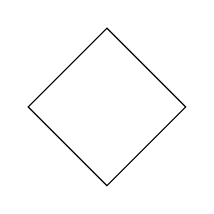
\begin{tikzpicture}
\draw (1,0) -- (0,1) -- (-1,0) -- (0,-1) -- cycle;
\end{tikzpicture}
\end{Verbatim}

\tikz{\draw (1,0) -- (0,1) -- (-1,0) -- (0,-1) -- cycle;}

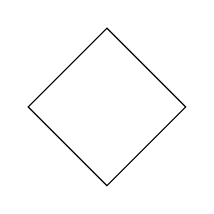
\begin{tikzpicture}
\draw (1,0) -- (0,1) -- (-1,0) -- (0,-1) -- cycle;
\end{tikzpicture}

有两种使用方法,一种命令式的,一种环境式的。命令式用tikz命令包围起来,命令式是inline模式的。环境式用tikzpicture命令包围起来。

这里推荐KTikZ软件,在ubuntu软件中心里面就有,用这个软件可以边写tikz代码边看画的图形,还可以导出图形,早期推荐先使用这个软件练练手熟悉下tikz制图代码。值得一提的是这个软件不支持中文注释,会生成乱码。



\chapter{tikz基础}

\section{tikz系统简介}
一般使用frontend layer(前端)就够了,有时可能需要用到basic layer(基本层)的命令。基本层是架构在系统层上的,里面是画图的最底层的驱动,绝大多数用户完全不需要了解这些。

tikz的画图命令要某在\verb+\tikz{}+里面,要某在tikzpicture环境里面。

\section{单位}
默认的长度单位是cm。



\section{第一个例子}
\subsection{画网格}
\begin{Verbatim}

\begin{tikzpicture}
\draw[step=1,color=gray!40] (-2,-2) grid (2,2);
\end{tikzpicture}
\end{Verbatim}


\begin{tikzpicture}
\draw[step=1,color=gray!40] (-2,-2) grid (2,2);
\end{tikzpicture}

step是网格之间的间距,color是网格的颜色。第一个坐标点是网格的左底点,第二个坐标点是网格的右顶点。我们可以看到tikzpicture下每一条命令最后都要跟一个分号\emph{;}。

\subsection{画直线}
\begin{Verbatim}
\begin{tikzpicture}
\draw[step=1,color=gray!40] (-2,-2) grid (2,2);
\draw (-3,0) -- (3,0);
\draw (0,-3) -- (0,3);
\end{tikzpicture}
\end{Verbatim}

\begin{tikzpicture}
\draw[step=1,color=gray!40] (-2,-2) grid (2,2);
\draw (-3,0) -- (3,0);
\draw (0,-3) -- (0,3);
\end{tikzpicture}

画直线就是两个坐标点相连,中间 -{}-{} 符号表示直线的意思。之前网格是grid表示网格的意思。

如果几个点用 -{}-{} 符号连接起来,表示这几个点连着来画几条折线,有多个画直线命令依次执行的意思。

\subsubsection{直线带上箭头}
draw命令可以跟上可选项\textbf{->},这样直线的右端就有一个箭头了。此外还有:\textbf{->>},\textbf{->|},\textbf{-to},\textbf{-latex},\textbf{-stealth}。

他们的效果从上到下依次演示如下:

\begin{tikzpicture}
\draw[->] (-3,3) -- (3,3);
\draw[->>] (-3,2) -- (3,2);
\draw[->|] (-3,1) -- (3,1);
\draw[-to] (-3,0) -- (3,0);
\draw[-latex] (-3,-1) -- (3,-1);
\draw[-stealth] (-3,-2) -- (3,-2);
\end{tikzpicture}

类似的还有左端比如\textbf{<-},或者两端比如\textbf{latex-latex},这里就不多说了。

\subsection{画圆}
接著上面的图案画一个圆,加入了以下代码:\\
\verb+\draw (0,0) circle (1); +

\begin{tikzpicture}
\draw[step=1,color=gray!40] (-2,-2) grid (2,2);
\draw[->] (-3,0) -- (3,0);
\draw[->] (0,-3) -- (0,3);
\draw (0,0) circle (1); 
\end{tikzpicture}

其中第一个点是圆中心,circle表示画圆,第二个参数是半径大小。


\subsection{画椭圆}
接著画一个椭圆:\\
\verb+\draw (0,0) ellipse (1 and 0.5);+

\begin{tikzpicture}
\draw[step=1,color=gray!40] (-2,-2) grid (2,2);
\draw[->] (-3,0) -- (3,0);
\draw[->] (0,-3) -- (0,3);
\draw (0,0) ellipse (1 and 0.5);
\end{tikzpicture}

这里第一个点是椭圆的中心点,ellipse表示画椭圆,后面参数两个值第一个是a也就是椭圆的半长轴,第二个是b也就是椭圆的半短轴。


\subsection{画弧线}

\begin{Verbatim}
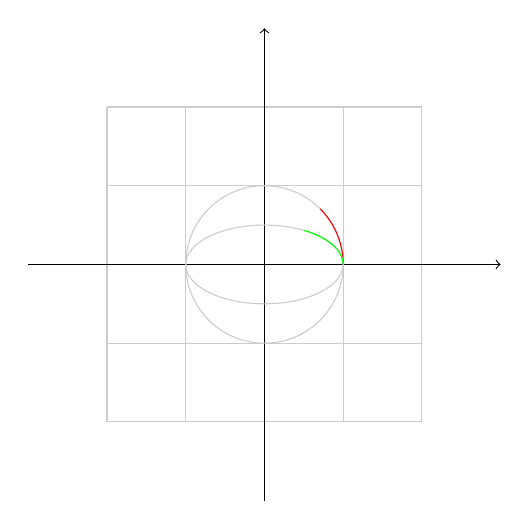
\begin{tikzpicture}
\draw[step=1,color=gray!40] (-2,-2) grid (2,2);
\draw[->] (-3,0) -- (3,0);
\draw[->] (0,-3) -- (0,3);
\draw[color=gray!40] (0,0) circle (1); %
\draw[color=red] (1,0) arc (0:45:1);
\draw[color=gray!40] (0,0) ellipse (1 and 0.5);
\draw[color=green] (1,0) arc (0:60:1 and 0.5);
\end{tikzpicture}
\end{Verbatim}
最基本的画弧线的命令如上代码第5行,其中第一个点是弧线的起点,然后arc表示画弧线,接下来括号里面的三个参数:第一个参数是开始的角度,第二个参数是结束时的角度,第三个参数是弧线对应圆的半径。对比第4行画的浅灰色的圆可以看出他们之间的关系。

上面代码第7行画弧线增加了一个and 和一个参数,这个时候画的弧线是根据椭圆来的,其中1是椭圆的半长轴,0.5是椭圆的半短轴。对比第6行画的浅灰色的椭圆可以看出他们的关系。

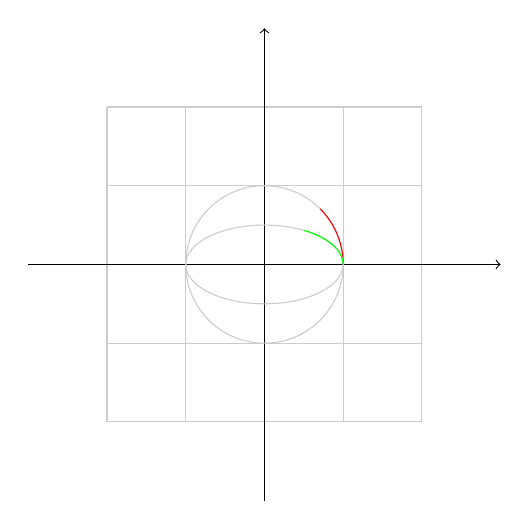
\begin{tikzpicture}
\draw[step=1,color=gray!40] (-2,-2) grid (2,2);
\draw[->] (-3,0) -- (3,0);
\draw[->] (0,-3) -- (0,3);
\draw[color=gray!40] (0,0) circle (1); %
\draw[color=red] (1,0) arc (0:45:1);
\draw[color=gray!40] (0,0) ellipse (1 and 0.5);
\draw[color=green] (1,0) arc (0:60:1 and 0.5);
\end{tikzpicture}



\subsection{点的定义}
tikz中定义一个点方便之后使用:

\begin{Verbatim}
\path (1,1) coordinate (point001);
\path (2,0) coordinate (point002);
\draw[dotted] (point001) -- (point002)  ;
\end{Verbatim}

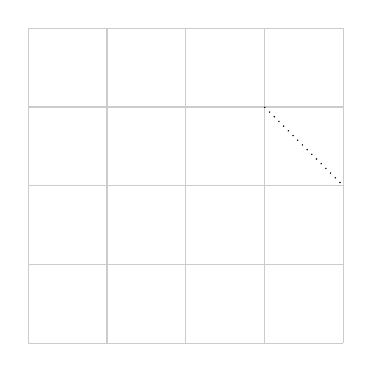
\begin{tikzpicture}
\draw[step=1,color=gray!40] (-2,-2) grid (2,2);
\path (1,1) coordinate (point001);
\path (2,0) coordinate (point002);
\draw[dotted] (point001) -- (point002)  ;
\end{tikzpicture}

这里代码的第6,7行定义了两个点,名字叫做point001和point002。然后用这两个点作为参数画了一个直线,这个直线有可选项\textbf{dotted},点线样式。

\subsection{放大图形}
在tikzpicture环境后面跟上可选项[scale=2],即将图形放大两倍。注意控制别越界了。

\begin{tikzpicture}[scale=2]
\draw[step=1,color=gray!40] (-2,-2) grid (2,2);
\draw[->] (-3,0) -- (3,0);
\draw[->] (0,-3) -- (0,3);
\end{tikzpicture}


\subsection{点的相对偏移}
现在加上这样两行代码:

\begin{Verbatim}
\draw[<->] (0,-2) -- ++(-1,1) -- ++(-1,-1);
\draw[dashed] (0,1) -- +(-1,1) -- +(-2,0);
\end{Verbatim}

\begin{tikzpicture}[scale=2]
\draw[step=1,color=gray!40] (-2,-2) grid (2,2);
\draw[latex-latex] (0,-2) -- ++(-1,1) -- ++(-1,-1);
\draw[dashed] (0,1) -- +(-1,1) -- +(-2,0);
\end{tikzpicture}

tikz中有一个重要的概念,当前点,然后点可以通过当前点根据相对偏移来确定一个新的点。上面代码第9行的\textbf{++}符号和第10行的\textbf{+}符号都根据当前点然后进行了$ \Delta x $和$ \Delta y $的相对偏移从而确定了一个新的点。这两个符号的区别在于是不是更新当前点数据。++符号更新当前点,而+符号不更新。


\subsection{画长方形}
现在加上这一行代码来画一个长方形:\\
\verb+\draw[color=red] (-1,-1) rectangle (1,1);+

\begin{tikzpicture}[scale=2]
\draw[step=1,color=gray!40] (-2,-2) grid (2,2);
\draw[color=red] (-1,-1) rectangle (1,1);
\end{tikzpicture}

这里使用了可选项\textbf{color=red}来控制线条的颜色,然后画长方形的第一个点是左底点,rectangle表示画长方形,第二个点表示右顶点。


\subsection{画函数}
画函数的功能是通过外部程序gnuplot来实现了,所以需要打开\verb+--shell-escape+,或者\verb+--enable-write18+

这里最后加了一个语句:\\
\verb+\draw[domain=-pi:pi,color=green] plot function{sin(x)};+

\begin{tikzpicture}[scale=1.8]
\draw[step=1,color=gray!40] (-2,-2) grid (2,2);
\draw[->] (-3,0) -- (3,0);
\draw[->] (0,-3) -- (0,3);
\draw (0,0) circle (1); %
\draw (0,0) ellipse (1 and 0.5);
\path (1,1) coordinate (point001);
\path (2,0) coordinate (point002);
\draw[dotted] (point001) -- (point002)  ;
\draw[<->] (0,-2) -- ++(-1,1) -- ++(-1,-1);
\draw[dashed] (0,1) -- +(-1,1) -- +(-2,0);
\draw[color=red] (-1,-1) rectangle (1,1);
\draw[domain=-pi:pi,color=green] plot function{sin(x)};
\end{tikzpicture}

这里可选项\textbf{domain=-pi:pi}控制画的函数的x范围,可以直接用pi表示π,然后接下来plot function表示画一个函数,接下来的花括号里面放着gnuplot的各种命令,这里就是简单的$ sin(x) $

\section{定义style}
\subsection{help lines}
\begin{Verbatim}
\tikzset{help lines/.style= {step=0.5cm,color=gray!40,very thin}}

\begin{tikzpicture}
\draw[help lines] (0,0) grid (5,5);
\end{tikzpicture}
\end{Verbatim}

\tikzset{help lines/.style= {step=0.5cm,color=gray!40,very thin}}

\begin{tikzpicture}
\draw[help lines] (0,0) grid (5,5);
\end{tikzpicture}

\subsection{information text}
\tikzset{information text/.style={rounded corners,fill=red!10,inner sep=1ex}}

\begin{tikzpicture}
\node[right, text width = 6cm,information text] {这是一段测试文字。};
\end{tikzpicture}



\section{颜色填充}
fill命令就是填充某种颜色的形状,后面跟个\textbf{color}可选项设置填充的颜色,默认是黑色。比如画一个填充颜色的圆:\\
\verb+\fill[cyan] (0,0) circle  (1) ;+

\newcommand{\testtext}{this is a test line}


\begin{tikzpicture}
\fill[cyan] (0,0) circle  (1) ;
\end{tikzpicture}

为了简单起见,draw命令可以加上fill可选项,然后和上面类似的有:

\begin{Verbatim}
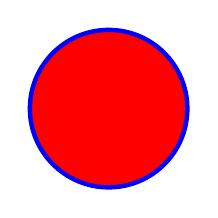
\begin{tikzpicture}
\draw [color=blue,fill=red,ultra thick,] (0,0) circle (1);
\end{tikzpicture}
\end{Verbatim}


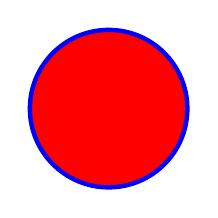
\begin{tikzpicture}
\draw [color=blue,fill=red,ultra thick,] (0,0) circle (1);
\end{tikzpicture}
注意到线条的颜色和填充颜色的控制。


\subsection{填充没有线条}
如果你不希望有线条,那么使用path命令可以做到这点。

\begin{Verbatim}

\begin{tikzpicture}
\path[fill=cyan] (0,0) circle  (1) ;
\end{tikzpicture}
\end{Verbatim}


\begin{tikzpicture}
\path[fill=cyan] (0,0) circle  (1) ;
\end{tikzpicture}


\section{clip命令}
clip就是剪切的意思,就是通过clip命令按照某个形状来剪切,外面的图形都不保留,可以跟一个可选项\textbf{draw},这样剪切的时候同时画出了这个形状。





\section{path路径闭合}
任何构建的path最后都可以通过\textbf{ -{}- cycle}将其闭合起来。

\section{filldraw命令}
是draw命令和fill命令的结合。\textbf{fill=}可选项调整填充的颜色,\textbf{draw=}可选项调整画的线条的颜色。

\section{阴影}
shade命令和fill命令的区别就是填充的颜色是渐变的,其他类似。

其可选项有\textbf{top color和bottom color}表示上下渐变的颜色,\textbf{left color和right color},\textbf{innercolor和outercolor},这些是配对的。此外还有\textbf{ball color}让颜色渐变像一个有光照的球。

\subsection{小红球}
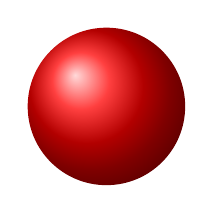
\begin{tikzpicture}
\shade[ball color=red] (1,2) circle (1);
\end{tikzpicture}


\section{scope环境}
scope环境就是作用域控制,一个局域环境,参数只影响内部,外部的参数也影响不进来,不过值得一提的是,定义的点外面也可以用。

scope环境一个有用的特性的里面的clip命令不会影响到外面。



\section{变形}
\textbf{xshift},x坐标轴平移。 \textbf{yshift},y坐标轴平移。\textbf{rotate},旋转 。\emph{注意xshift默认的单位并不是cm,如果要单位是cm需要写出来。}

\subsection{旋转图形}
后面加上可选项\textbf{rotate=30}即可,意思是图形逆时针旋转30度。

\begin{Verbatim}
\begin{tikzpicture}
\draw (0,0)[rotate=30]  ellipse (2 and 1);
\end{tikzpicture}
\end{Verbatim}

\begin{tikzpicture}
\draw (0,0)[rotate=30]  ellipse (2 and 1);
\end{tikzpicture}




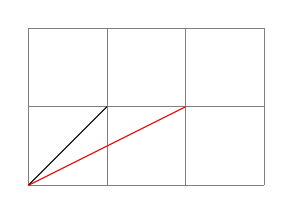
\begin{tikzpicture}
\draw[help lines] (0,0) grid (3,2);
\draw (0,0) -- (1,1);
\draw[red] (0,0) -- ([xshift=1cm] 1,1);
\end{tikzpicture}

\section{迭代语句}
\begin{Verbatim}
\begin{tikzpicture}
\draw[help lines] (0,0) grid (3,2);
\foreach \x in {0,1,...,4}
\draw[xshift=\x cm] (0,-1) -- (0,1);
\end{tikzpicture}
\end{Verbatim}

\begin{tikzpicture}
\draw[help lines] (0,0) grid (3,2);
\foreach \x in {0,1,...,4}
\draw[xshift=\x cm] (0,-1) -- (0,1);
\end{tikzpicture}

其中...表示一直这样有规律下去生成迭代列表。迭代语句有很多用法,详见后面的具体例子。






\section{baseline选项}
这个主要控制inline模式下图片的位置,默认\textbf{baseline=0pt}。

\section{样式}
style,特定图形的样式。定义一个样式比如style001如下:\\
\verb+style001/.style={color=red,fill=red!20}+

\subsection{原有样式修改}
\verb+help lines/.append style=blue!50+\\
附加之后最新的样式胜出。

\subsection{样式带参数}
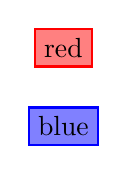
\begin{tikzpicture}[outline/.style={draw=#1,thick,fill=#1!50}]
\node [outline=red] at (0,1) {red};
\node [outline=blue] at (0,0) {blue};
\end{tikzpicture}

\subsection{样式参数有默认值}
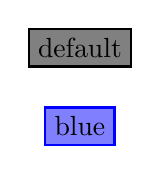
\begin{tikzpicture}[outline/.style={draw=#1,thick,fill=#1!50},
outline/.default=black]
\node [outline]
at (0,1) {default};
\node [outline=blue] at (0,0) {blue};
\end{tikzpicture}

\section{定义点}
\subsection{定义绝对点}
\begin{Verbatim}
\path (0,29) coordinate (top-left);
\end{Verbatim}
path命令后面跟着坐标点,然后coordinate后面跟着这个点的名字。这里规范为coordinate命令后面跟着就是点的名字,node命令后面跟着node的名字。

\subsection{定义相对点}
\begin{Verbatim}
\path (top-left) ++(1,-2) coordinate (name-point);
\end{Verbatim}

++适合描述一连串逐渐变化的点,+适合描述多个点围绕着一个点变化的情况。
\subsection{极座标}
tikz中的点也支持极座标表示,(30:1cm),第一个参数是极座标里面的角度,第二个参数是半径。


\subsection{node命令中点的定义}

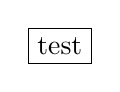
\begin{tikzpicture}
\node (node001) at (0,2) [draw] {test};
\end{tikzpicture}

从这里可以看到只要写上draw选项外面就会加上一个长方形,也就是shape的默认选项是rectangle。如果你不希望外面有长方形,不写draw选项即可。

这里通过node命令定义了一个点,node001,在(0,2)那里。后面是可以使用的。

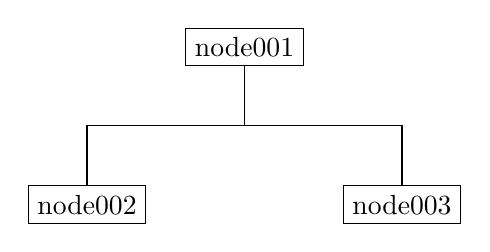
\begin{tikzpicture}
\node (node001) at (0,2) [draw] {node001};
\node (node002) at (-2,0) [draw] {node002};
\node (node003) at (2,0) [draw] {node003};
\draw (node cs:name=node003,anchor=north) |- (0,1);
\draw (node002.north) |- (0,1) -| (node cs:name=node001,anchor=south);
\end{tikzpicture}

这里通过\textbf{node cs:name=node003}来获取之前那个node所在的点,然后通过\textbf{anchor=north}来定义那个node的接口在北边。除此之外的选项还有:\textbf{south},\textbf{east},\textbf{west}。这里\textbf{|-}似乎是画垂直拐线的意思。上面的语法简写为可以node002.north。

此外还有\textbf{angle}选项控制node接口的开口角度。

\subsection{两个点定义出一个点}
\begin{Verbatim}
\begin{tikzpicture}
\node (p1) at (30:1) {$p_1$} ;
\node (p2) at (75:1) {$p_2$} ;
\draw (-0.2,0) -- (1.2,0) node[right] (xline) {$q_1$};
\draw (2,-0.2) -- (2,1.2) node[above] (yline) {$q_2$};

\draw[->] (p1) -- (p1 |- xline);
\end{tikzpicture}
\end{Verbatim}

这种形式(p1 |- xline)表示取第一个点的x和第二个点的y组成一个新的点。如果是(p1 -| xline)表示取第二个点的x和第一个点的y组成一个新的点。

\begin{tikzpicture}
\node (p1) at (30:1) {$p_1$} ;
\node (p2) at (75:1) {$p_2$} ;
\draw (-0.2,0) -- (1.2,0) node[right] (xline) {$q_1$};
\draw (2,-0.2) -- (2,1.2) node[above] (yline) {$q_2$};

\draw[->] (p1) -- (p1 |- xline);
\end{tikzpicture}



\subsection{两个path的交点}
\begin{Verbatim}
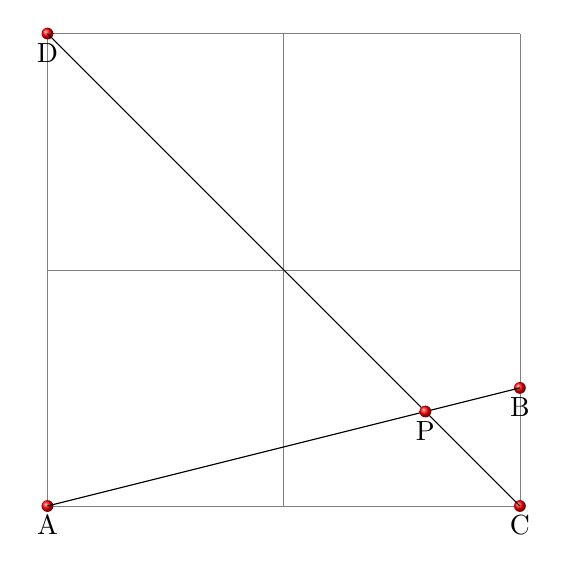
\begin{tikzpicture}[scale=3]
\draw[help lines] (0,0) grid (2,2);
\coordinate (A) at (0,0);
\coordinate (B) at (2,0.5);
\coordinate (C) at (2,0);
\coordinate (D) at (0,2);
\shade[ball color=red](A) circle (0.025) node[below] {A};
\shade[ball color=red](B) circle (0.025) node[below] {B};
\shade[ball color=red](C) circle (0.025) node[below] {C};
\shade[ball color=red](D) circle (0.025) node[below] {D};
\draw[name path=AB] (A) -- (B);
\draw[name path=CD] (C) -- (D);
\path[name intersections={of=AB and CD}] (intersection-1) coordinate (P);
\shade[ball color=red](P) circle (0.025) node[below] {P};
\end{tikzpicture}
\end{Verbatim}


\usetikzlibrary{intersections,calc}
\tikzset{help lines/.style= {step=0.5cm,color=gray!40,very thin}}
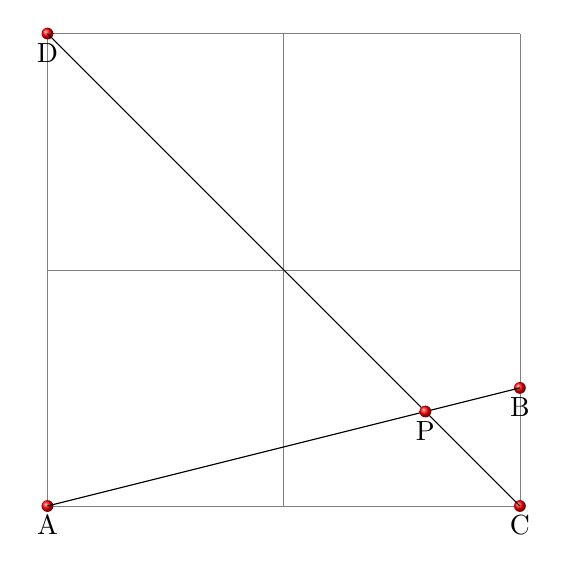
\begin{tikzpicture}[scale=3]
\draw[help lines] (0,0) grid (2,2);
\coordinate (A) at (0,0);
\coordinate (B) at (2,0.5);
\coordinate (C) at (2,0);
\coordinate (D) at (0,2);
\shade[ball color=red](A) circle (0.025) node[below] {A};
\shade[ball color=red](B) circle (0.025) node[below] {B};
\shade[ball color=red](C) circle (0.025) node[below] {C};
\shade[ball color=red](D) circle (0.025) node[below] {D};
\draw[name path=AB] (A) -- (B);
\draw[name path=CD] (C) -- (D);
\path[name intersections={of=AB and CD}] 
(intersection-1) coordinate (P);
\shade[ball color=red](P) circle (0.025) node[below] {P};
\end{tikzpicture}

这个例子用到了点的定义,点的标出,以及path交点的定义,要用到library:\textbf{intersections}。有时候有些路径你不希望显示出来那么就用path命令来定义路径。

\subsubsection{给新交点取名字}
用\textbf{by}选项可以给画出来的交点取一个名字,默认的\\intersection-1之类的也可以使用。此外还可以加上选项:
\begin{Verbatim}
\path [name intersections={of=D and E, 
by={[label=above:$C$]C, [label=below:$C'$]C'}}];
\end{Verbatim}



\subsection{点的运算}
在进行下面说的数学运算之前需要加载calc宏包:\\
\verb+\usetikzlibrary{calc}+

基本格式是:\\
\verb+([options]$(一些运算)$)+

这里\verb+$$+表示这里有一些数学运算。里面的基本格式如下:\\
\verb+<factor>*<点><其他修饰>+

\begin{Verbatim}
\begin{tikzpicture}[scale=3]
\draw [help lines] (0,0) grid (3,2);
\fill [red] ($2*(1,1)$) circle (2pt);
\fill [green] (${1+1}*(1,0.5)$) circle (2pt);
\fill [blue] ($cos(0)*sin(90)*(1,1)$) circle (2pt);
\fill [black] (${3*(4-3)}*(1,0.5)$) circle (2pt);
\end{tikzpicture}
\end{Verbatim}

第一个红点是点(1,1),然后x和y都乘以2从而得到新点。后面情况类似,不同的是前面的乘法还可以加入更多的运算。

\begin{tikzpicture}[scale=3]
\draw [help lines] (0,0) grid (3,2);
\fill [red] ($2*(1,1)$) circle (2pt);
\fill [green] (${1+1}*(1,0.5)$) circle (2pt);
\fill [blue] ($cos(0)*sin(90)*(1,1)$) circle (2pt);
\fill [black] (${3*(4-3)}*(1,0.5)$) circle (2pt);
\end{tikzpicture}

这里有点类似矢量运算计算出点的位置,前面计算出乘量因子,然后后面一个矢量偏移量。


\section{计算两个点之间的距离}
\begin{Verbatim}
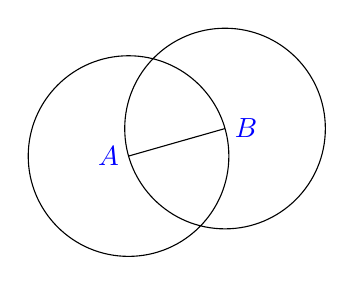
\begin{tikzpicture}
\coordinate[label=left:\textcolor{blue}{$A$}] (A) at ($(0,0) +0.1*(rand,rand)$) ;
\coordinate[label=right:\textcolor{blue}{$B$}] (B) at ($(1.25,0.25) +0.1*(rand,rand)$) ;

\draw (A) -- (B);

\draw  let
\p1 = ($ (B) - (A) $),
\n1 = {veclen(\x1,\y1)}
in
(A) circle (\n1)
(B) circle (\n1);

\end{tikzpicture}
\end{Verbatim}

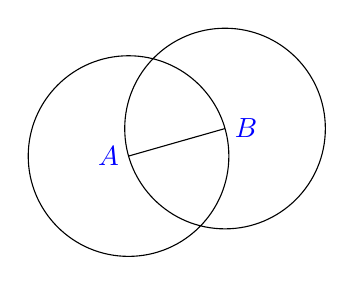
\begin{tikzpicture}
\coordinate[label=left:\textcolor{blue}{$A$}] (A) 
at ($(0,0) +0.1*(rand,rand)$) ;
\coordinate[label=right:\textcolor{blue}{$B$}] (B)
 at ($(1.25,0.25) +0.1*(rand,rand)$) ;

\draw (A) -- (B);

\draw  let
\p1 = ($ (B) - (A) $),
\n1 = {veclen(\x1,\y1)}
in
(A) circle (\n1)
(B) circle (\n1);

\end{tikzpicture}

\textbf{let ... in ...}语句可以放在任何path命令的任何位置来控制变量的计算和定义。
\textbackslash p\textit{<digit>}定义的是点的变量,\textbackslash n\textit{<digit>}定义的是数值的变量,后面可以跟数字从而定义多个变量。

任何点变量都可以用\textbackslash x\textit{<digit>}和\textbackslash y\textit{<digit>}来引用该点的x坐标和y坐标。

\textbf{veclen}函数计算某个矢量的长度。



\section{path之线条}
path路径是最基本的命令,draw命令等价于\verb+\path[draw]+,fill命令等价于\verb+\path[fill]+,filldraw命令等价于\verb+\path[draw,fill]+,其他clip,shade命令情况类似。

\subsection{虚线和点线}
线条除了之前说的dashed和dotted两种样式之外,还有loosely dashed,densely dashed和loosely dotted, densely dotted。比如:\tikz{\draw[loosely dashed] (0,0) -- (1,0);} ~~ \tikz{\draw[dashed] (0,0) -- (1,0);} ~~ \tikz{\draw[densely dashed] (0,0) -- (1,0);},这是dashed的三种,下面是dotted的三种:\tikz{\draw[loosely dotted] (0,0) -- (1,0);} ~~ \tikz{\draw[dotted] (0,0) -- (1,0);} ~~ \tikz{\draw[densely dotted] (0,0) -- (1,0);}。

\subsection{线条的粗细}
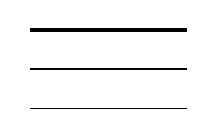
\begin{tikzpicture}
\draw [ultra thick] (0,1) -- (2,1);
\draw [thick] (0,0.5) -- (2,0.5);
\draw [thin] (0,0) -- (2,0);
\end{tikzpicture}

其他选项还有\textbf{ultra thin}, \textbf{very thin}, \textbf{thin}, \textbf{semithick},  \textbf{thick},\\ \textbf{very thick} and \textbf{ultra thick}
还有\textbf{help lines}选项那种很淡灰的样式。

或者直接通过可选项line width来定义。


\begin{tikzpicture}
\draw [line width=12] (0,0) -- (2,0);
\draw [line width=0.2cm] (4,.75) -- (5,.25);
\end{tikzpicture}


\subsection{圆圆的拐角}
\begin{tikzpicture}
\draw [<->, rounded corners, thick, purple] (0,2) -- (0,0) -- (3,0);
\end{tikzpicture}

\section{贝塞尔曲线}
贝塞尔曲线是四个点画出一个曲线,具体我现在还不太清楚。其中第一个点是起点,第四个点终点,然后另外两个点是控制点。

\begin{Verbatim}
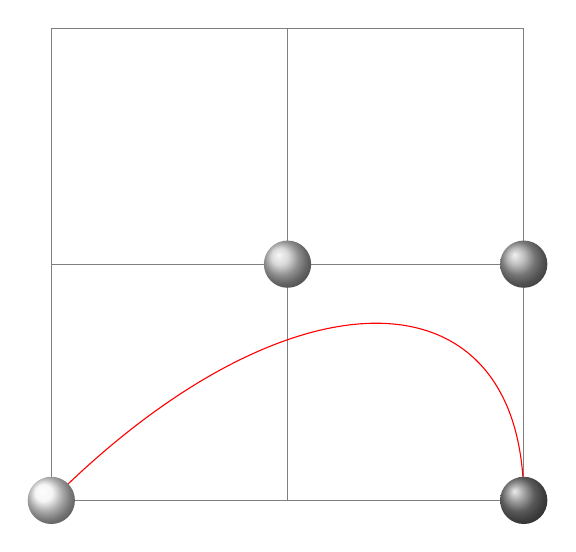
\begin{tikzpicture}[scale=3]
\draw[help lines] (0,0) grid (2,2);
\draw[color=red] (0,0) .. controls (1,1) and (2,1) .. (2,0);
\shade[ball color=gray!10] (0,0) circle (0.1);
\shade[ball color=gray!40] (1,1) circle (0.1);
\shade[ball color=gray!70] (2,1) circle (0.1);
\shade[ball color=gray] (2,0) circle (0.1);
\end{tikzpicture}
\end{Verbatim}

上面第2行代码就是画贝塞尔曲线的代码。

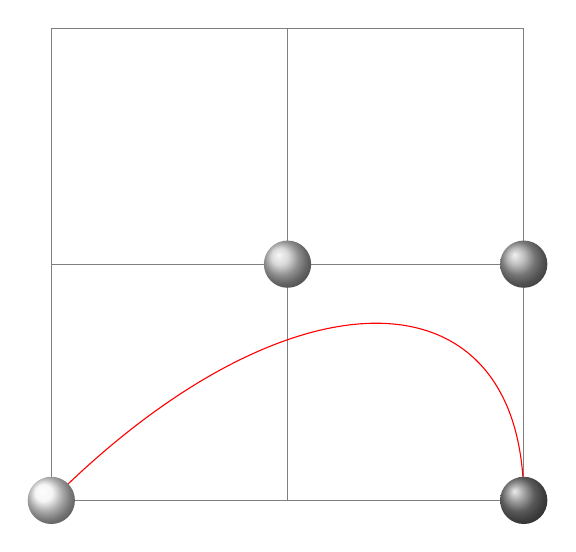
\begin{tikzpicture}[scale=3]
\draw[help lines] (0,0) grid (2,2);
\draw[color=red] (0,0) .. controls (1,1) and (2,1) .. (2,0);
\shade[ball color=gray!10] (0,0) circle (0.1);
\shade[ball color=gray!40] (1,1) circle (0.1);
\shade[ball color=gray!70] (2,1) circle (0.1);
\shade[ball color=gray] (2,0) circle (0.1);
\end{tikzpicture}



\section{弧线}
\subsection{弧线反向}
\begin{Verbatim}
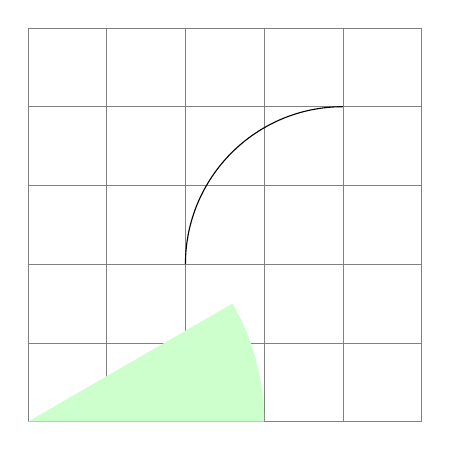
\begin{tikzpicture}
\draw[help lines] (0,0) grid (5,5);
\fill[green!20] (0,0) -- (3,0)
arc (0:30:3)  -- cycle;
\draw (2,2) arc (0:-90:-2);
\end{tikzpicture}
\end{Verbatim}


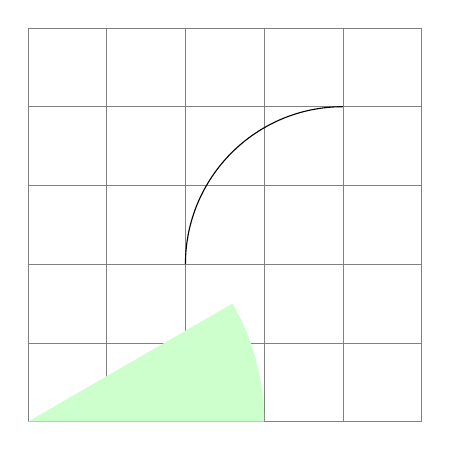
\begin{tikzpicture}
\draw[help lines] (0,0) grid (5,5);
\fill[green!20] (0,0) -- (3,0)
arc (0:30:3)  -- cycle;
\draw (2,2) arc (0:-90:-2);
\end{tikzpicture}

我们可以看到画弧线如果要中心点不是在左边而是在右边,那么可以通过让半径为负值和调整角度获得。其中角度的计算是顺时针的负值。




\section{node命令}
node命令主要用于插入文本,不过最好将其理解为接口。\XeLaTeX 文档内部各个命令等都可以使用,然后外面包围一个形状,如rectangle长方形,circle圆等。

\begin{Verbatim}
\newcommand{\testlinea}{this is a test line a}
\newcommand{\testlineb}{this is a test line b}
\begin{tikzpicture}
%\fill[cyan] (0,0) circle  (1) ;
\node[shape=rectangle,draw,inner sep=10pt] at (0,0) (a) {\testlinea};
\node[shape=rectangle,draw,inner sep=10pt] at (0,-3) (b) {\testlineb};
\draw[-latex](a) -- (b);
\end{tikzpicture}
\end{Verbatim}

这里我们看到\LaTeX 里面自定义的命令是可以正常使用的,然后可选项\textbf{shape}的意思是外面包围的形状是长方形,\textbf{draw}就是画这个形状是用的draw命令方法,比如fill就会填充。\textbf{inner sep}控制外面的形状和内部文本之间的间距。 然后\textbf{at (0,0)}控制整个图形的位置,然后\textbf{(a)}表示整个图形的名字,后面可以调用的,可以看作接口把。然后后面就是\LaTeX 的内容了。

\newcommand{\testlinea}{this is a test line a}
\newcommand{\testlineb}{this is a test line b}
\begin{tikzpicture}
%\fill[cyan] (0,0) circle  (1) ;
\node[shape=rectangle,draw,inner sep=10pt] at (0,0) (a) {\testlinea};
\node[shape=rectangle,draw,inner sep=10pt] at (0,-3) (b) {\testlineb};
\draw[-latex](a) -- (b);
\end{tikzpicture}

\subsection{插入文本的位置}
node命令的可选项\textbf{left},\textbf{right},\textbf{above},\textbf{below}用于控制插入文本的位置。此外还有\textbf{above right},\textbf{below right},\textbf{above left} ,\textbf{below left}等。

\subsection{文本对齐控制}
用\textbf{align=left},\textbf{align=right},\textbf{align=center}来控制。

\subsection{在画图形的时候插入文本}
\begin{tikzpicture}
\draw (1,1) node {text} -- (2,2);
\end{tikzpicture}

在画图形的时候某个当前点下可以直接node接某个文本。

node命令在path的任何位置都可插入,具体是path完成之后才绘制出node要插入的内容。

node的\textbf{inner sep}选项调整node文本和外围的shape之间的间距。

node的\textbf{minimum size}选项控制node没有文本时候外围shape的大小,装上文本可以更大。

node可以通过\textbf{at}来具体控制node的位置,可以通过\textbf{[below=of wating]}这样的语句来让新的node相对其他node而存在。


\subsection{node旁插入标签}
node旁边加上标签,使用\textbf{label}选项,语法是:\\
\verb+label=above:$s\le3$+。除了常用的above,below等控制位置外,还可以直接用60这样的数值控制位置,表示node圆圈逆时针旋转60度的那个位置。

所有标签的样式可以通过重定义\textbf{every label}样式来实现,


\subsection{node用箭头连接}
\verb+\draw [->] (critical.west) -- (enter critical.east);+
比如上面这个语句,critical是node的名字,\emph{.west}表示该node的shape的西边(也就是左边)出发。

\subsection{弯曲箭头}
用\textbf{to}语句更加灵活地画弯曲箭头,out选项控制出来的角度,in选项控制进去的角度。
\textbf{bend right}选项很有用,此外还有\textbf{bend left}选项,后面跟数值控制偏转量,一般45。

\subsection{箭头旁边加标签}
to语句后面跟个node就可以直接加上标签,表示在这个箭头path上加个node。这种方法有一个\textbf{swap}可以让标签交换位置。


\subsection{shape穿过某个点}
使用through包可以让node外的某个shape自定义穿过某个点,比如\textbf{circle through}=(3,3)




\section{tikz中的随机数}
\textbf{rand}产生一个随机数,范围在-1~1之间。




\chapter{tikz的一些例子}
\section{画正多边形}
\begin{Verbatim}

\begin{tikzpicture}
\draw (0,0) circle (4) ;
\coordinate (O) at (0,0);
\shade[ball color=red](O) circle (0.1) node[below] {O};
\def\n{5}
\pgfmathsetmacro\i{\n-1}
\foreach \x in {0,...,\i}
{
\def\pointname{\x}
\coordinate (\pointname) at ($(0,0) +(\x*360/\n:4cm)$)  ;
\shade[ball color=red](\pointname) circle (0.05) node[below] {\small \x};
}

\draw (0)
\foreach \x in {0,...,\i}
{ -- (\x) } -- cycle;

\end{tikzpicture}
\end{Verbatim}

\begin{tikzpicture}
\draw (0,0) circle (4) ;
\coordinate (O) at (0,0);
\shade[ball color=red](O) circle (0.1) node[below] {O};
\def\n{5}
\pgfmathsetmacro\i{\n-1}
\foreach \x in {0,...,\i}
{
\def\pointname{\x}
\coordinate (\pointname) at ($(0,0) +(\x*360/\n:4cm)$)  ;
\shade[ball color=red](\pointname) circle (0.05) node[below] {\small \x};
}

\draw (0)
\foreach \x in {0,...,\i}
{ -- (\x) } -- cycle;

\end{tikzpicture}

这个例子核心内容是批量定义点和点的运算,把这个弄懂了,后面tikz的核心大门就为你打开了,然后很多图形都可以用简洁的命令生成出来了。


\section{多个node连接}
\begin{Verbatim}
\usetikzlibrary{positioning}
\tikzset{place/.style={circle,draw=blue!50,fill=blue!20,
thick,inner sep=0pt,minimum size=6mm}}
\tikzset{transition/.style={rectangle,draw=black!50,
fill=black!20,thick,inner sep=0pt,minimum size=4mm}}
\tikzset{every label/.style=red}
\begin{tikzpicture}[bend angle=45]
\node[place] (waiting)  {};
\node[place] (critical) [below=of waiting] {};
\node[place](semaphore) [below=of critical,label=above:$s\le3$] {};
\node[transition](leave critical) [right=of critical]{};
\node[transition] (enter critical)[left=of critical]{};
\draw [->] (enter critical) to (critical);
\draw [->] (waiting) to [bend right] (enter critical);
\draw [->] (enter critical) to [bend right] (semaphore);
\draw [->] (semaphore) to [bend right] (leave critical);
\draw [->] (critical) to (leave critical);
\draw [->] (leave critical) to [bend right] (waiting);
\end{tikzpicture}
\end{Verbatim}

\tikzset{place/.style={circle,draw=blue!50,fill=blue!20,thick,inner sep=0pt,minimum size=6mm}}
\tikzset{transition/.style={rectangle,draw=black!50,fill=black!20,thick,inner sep=0pt,minimum size=4mm}}
\tikzset{every label/.style=red}
\begin{tikzpicture}[bend angle=45]
\node[place] (waiting)  {};
\node[place] (critical) [below=of waiting] {};
\node[place](semaphore) [below=of critical,label=above:$s\le3$] {};
\node[transition](leave critical) [right=of critical]{};
\node[transition] (enter critical)[left=of critical]{};
\draw [->] (enter critical) to (critical);
\draw [->] (waiting) to [bend right] (enter critical);
\draw [->] (enter critical) to [bend right] (semaphore);
\draw [->] (semaphore) to [bend right] (leave critical);
\draw [->] (critical) to (leave critical);
\draw [->] (leave critical) to [bend right] (waiting);
\end{tikzpicture}

这个例子需要加载positioning包,这个例子很好地展示了多个node和用箭头连接来表示他们关系的图形如何绘制。


\section{几何第一个例子}
为了减少文档大小,我编写的tikz的例子都放入文件夹\emph{tikz制图}里面,可以用Ktikz软件直接打开查看。

\begin{Verbatim}

\begin{tikzpicture}
\coordinate[label=left:\textcolor{blue}{$A$}] (A) 
at ($(0,0) +0.1*(rand,rand)$) ;
\coordinate[label=right:\textcolor{blue}{$B$}] (B) 
at ($(1.25,0.25) +0.1*(rand,rand)$) ;

\draw [name path=A--B] (A) -- (B);

\node [name path=D,draw,circle through=(B),label=left:$D$] at (A) {};
\node [name path=E,draw,circle through=(A),label=right:$E$] at (B) {};

\path [name intersections={of=D and E, 
by={[label=above:$C$]C, [label=below:$C'$]C'}}];

\draw [red] (A) -- (C);
\draw [red] (B) -- (C);

\draw [name path=C--C',red] (C) -- (C');
\path [name intersections={of=A--B and C--C',by=F}];

\node [fill=red,inner sep=1,label=-45:$F$] at (F) {};

\foreach \point in {A,B,C,C'}
\fill [black,opacity=.5] (\point) circle (2pt);

\begin{pgfonlayer}{background}
\fill[orange!80] (A) -- (C) -- (B) -- cycle;
\end{pgfonlayer}

\end{tikzpicture}
\end{Verbatim}

\begin{tikzpicture}
\coordinate[label=left:\textcolor{blue}{$A$}] (A) at ($(0,0) +0.1*(rand,rand)$) ;
\coordinate[label=right:\textcolor{blue}{$B$}] (B) at ($(1.25,0.25) +0.1*(rand,rand)$) ;

\draw [name path=A--B] (A) -- (B);

\node [name path=D,draw,circle through=(B),label=left:$D$] at (A) {};
\node [name path=E,draw,circle through=(A),label=right:$E$] at (B) {};

\path [name intersections={of=D and E, by={[label=above:$C$]C, [label=below:$C'$]C'}}];

\draw [red] (A) -- (C);
\draw [red] (B) -- (C);

\draw [name path=C--C',red] (C) -- (C');
\path [name intersections={of=A--B and C--C',by=F}];

\node [fill=red,inner sep=1,label=-45:$F$] at (F) {};

\foreach \point in {A,B,C,C'}
\fill [black,opacity=.5] (\point) circle (2pt);

\begin{pgfonlayer}{background}
\fill[orange!80] (A) -- (C) -- (B) -- cycle;
\end{pgfonlayer}

\end{tikzpicture}


\section{数据点可视化}




\chapter{其他}
\section{文本中的图片}
wherever \begin{tikzpicture} \draw [yellow, line width=6]
(0,0) -- (.5,0); \end{tikzpicture} you want


%这里空一行

\end{common-format}
\end{document}



